\documentclass{article}

% if you need to pass options to natbib, use, e.g.:
%     \PassOptionsToPackage{numbers, compress}{natbib}
% before loading neurips_2024


% ready for submission
% \usepackage{neurips}


% to compile a preprint version, e.g., for submission to arXiv, add add the
% [preprint] option:
%     \usepackage[preprint]{neurips_2024}


% to compile a camera-ready version, add the [final] option, e.g.:
\usepackage[final]{neurips}


% to avoid loading the natbib package, add option nonatbib:
%    \usepackage[nonatbib]{neurips_2024}


\usepackage[utf8]{inputenc} % allow utf-8 input
\usepackage[T1]{fontenc}    % use 8-bit T1 fonts
\usepackage{hyperref}       % hyperlinks
\usepackage{url}            % simple URL typesetting
\usepackage{booktabs}       % professional-quality tables
\usepackage{amsfonts}       % blackboard math symbols
\usepackage{nicefrac}       % compact symbols for 1/2, etc.
\usepackage{microtype}      % microtypography
\usepackage{xcolor}         % colors
\usepackage{graphicx} % figures
\usepackage{float} % figures
\usepackage{amsmath, amsfonts, amssymb} % equations
\bibliographystyle{abbrvnat}


\title{Heat Kernel Smoothing}


% The \author macro works with any number of authors. There are two commands
% used to separate the names and addresses of multiple authors: \And and \AND.
%
% Using \And between authors leaves it to LaTeX to determine where to break the
% lines. Using \AND forces a line break at that point. So, if LaTeX puts 3 of 4
% authors names on the first line, and the last on the second line, try using
% \AND instead of \And before the third author name.


\author{
  Gabriel Riegner\\
  DSC 291 Network Science and Graph Theory
}


\begin{document}

\maketitle

\begin{abstract}
This report reviews and evaluates the paper "Heat Kernel Smoothing Using Laplace-Beltrami Eigenfunctions" by \citet*{seo_heat_2010}, with applications to brain cortical surface smoothing. We compare this method with iterative nearest-neighbor smoothing on a population-average FreeSurfer cortical surface mesh. Our analysis shows that heat kernel smoothing generates smooth random fields with spatial autocorrelation functions (ACFs) matching the kernel shape. Simulations validate that heat kernel smoothing outperforms iterative methods in approximating theoretical ACFs, with lower RMSE at both low and high smoothing levels. While iterative smoothing shows surprising accuracy despite lacking formal mathematical foundation, both methods display downward bias at high autocorrelations. This work provides a framework for generating random fields with controlled spatial properties on complex surfaces, essential for validating downstream statistical inference methods in neuroimaging.
\end{abstract}



\section{Introduction and Motivation}

Cortical surface analysis in neuroimaging requires methods that adapt to the brain’s intrinsic geometry. As shown in Figure \ref{fig:surface-data}, anatomical MRI data is translated into surface meshes through a series of steps that reconstruct the folded cortical geometry \citep{dale_cortical_1999}. However, for data obtained along curved non-Euclidean surfaces, traditional statistical analysis and smoothing techniques based in Euclidean space are inaccurate. Traditional Euclidean-based smoothing methods fail here because they ignore the surface’s curvature (Figure \ref{fig:surface-distances}A–C), where geodesic distances, that measure shortest paths along the folded surface, are anatomically more meaningful.\\

Heat kernel smoothing addresses this challenge by leveraging the eigenfunctions of the Laplace-Beltrami operator for smoothing on manifolds. When applied to uncorrelated noise, it generates smooth random fields whose autocorrelation function (ACF) exactly matches the heat kernel with double bandwidth ($2\sigma$), introducing spatially structured correlations that respect intrinsic geometry \citep{chung_cortical_2005}. This property enables precise control over spatial covariance structures (Figure \ref{fig:simulation-results}), critical for validating statistical inference methods in neuroimaging that rely on random field theory \citep{kushnarev_heat_2019}. By preserving both geometric fidelity and Gaussian assumptions, heat kernel smoothing provides a unified framework for denoising and simulating neuroimaging data on irregular domains.\\

However, open questions remain about the convergence properties of empirical smoothing methods and the optimal trade-offs between analytical precision and computational efficiency in real-world applications.

\begin{figure}[H]
    \centering
    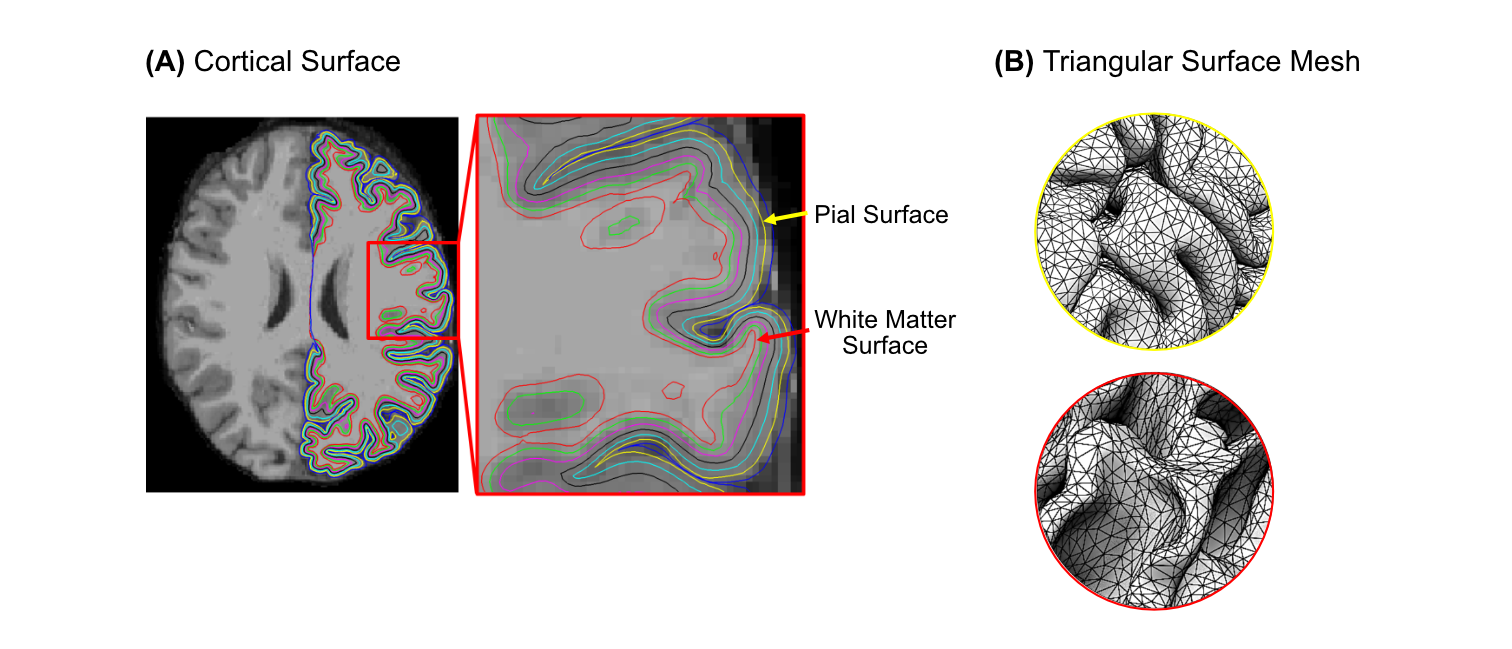
\includegraphics[width=0.9\linewidth]{project/figures/fig01.png}
    \caption{
    \textbf{(A)} Tissue segmentation of anatomical MRI, which separates gray matter boundary (pial surface) from white matter. 
    \textbf{(B)} After tissue segmentation, brain surfaces are discretized into triangular meshes ($\sim$40k vertices, $\sim$80k triangles per hemisphere), which can be treated as smooth Riemannian manifolds. 
    }
    \label{fig:surface-data}
\end{figure}

\begin{figure}[H]
    \centering
    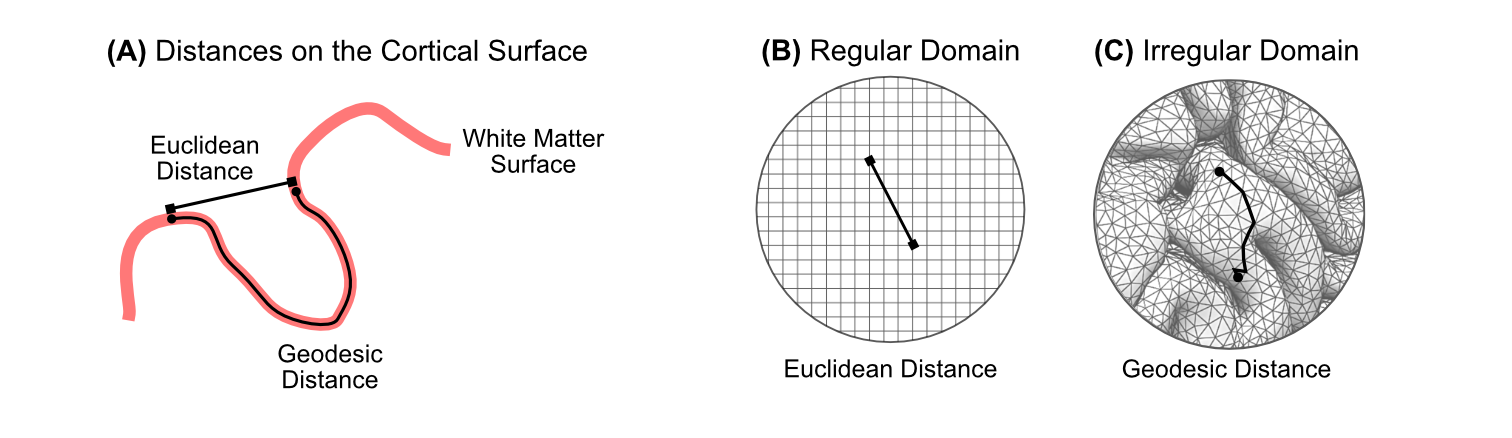
\includegraphics[width=0.9\linewidth]{project/figures/fig02.png}
    \caption{
    \textbf{(A)} Euclidean distance measure the straight-line separation between two points on the brain, ignoring the curvature of the cortical surface. In contrast, geodesic distance calculates the shortest path along the folded cortical surface preserving the underlying anatomy.
    \textbf{(B)} In regular domains (e.g. uniform grids), Euclidean distance suffices as it directly measures straight-line separation, assuming a flat uniform geometry. 
    \textbf{(C)} For irregular domains (e.g. cortical surfaces), geodesic distance accounts for intrinsic curvature and folding.
    }
    \label{fig:surface-distances}
\end{figure}


\section{Paper Overview}
\subsection{Problem Setting}

In medical imaging, anatomical data represented as triangular meshes contains noise introduced during segmentation, mesh construction, and geometric computations. Traditional methods for addressing this noise have significant limitations. Iterated kernel smoothing, widely used in computational anatomy and computer vision, spatially adapts kernel weights to follow the shape of the heat kernel in a discrete fashion along a manifold. This approach linearly approximates the heat kernel using the Gaussian kernel in the tangent space, but compounds linearization errors at each iteration, reducing accuracy with successive applications \citep{seo_heat_2010}.\\

Smoothing data defined on irregular domains such as the cortical surface presents unique challenges. Traditional Gaussian smoothing methods designed for Euclidean spaces often fail when applied to surfaces with folded geometry. Instead, isotropic heat diffusion is a generalization of Gaussian smoothing to irregular domains such as manifolds and graphs, which represents how heat would diffuse equally in all directions along a manifold \citep{kushnarev_heat_2019, seo_heat_2010, zhang_graph_2008, grigoryan_heat_2012}. Locally, the heat kernel behaves like a Gaussian kernel. Globally, the heat kernel adapts to the irregular domain by following geodesic distances, thereby preserving anatomical relationships.\\


\begin{figure}[H]
    \centering
    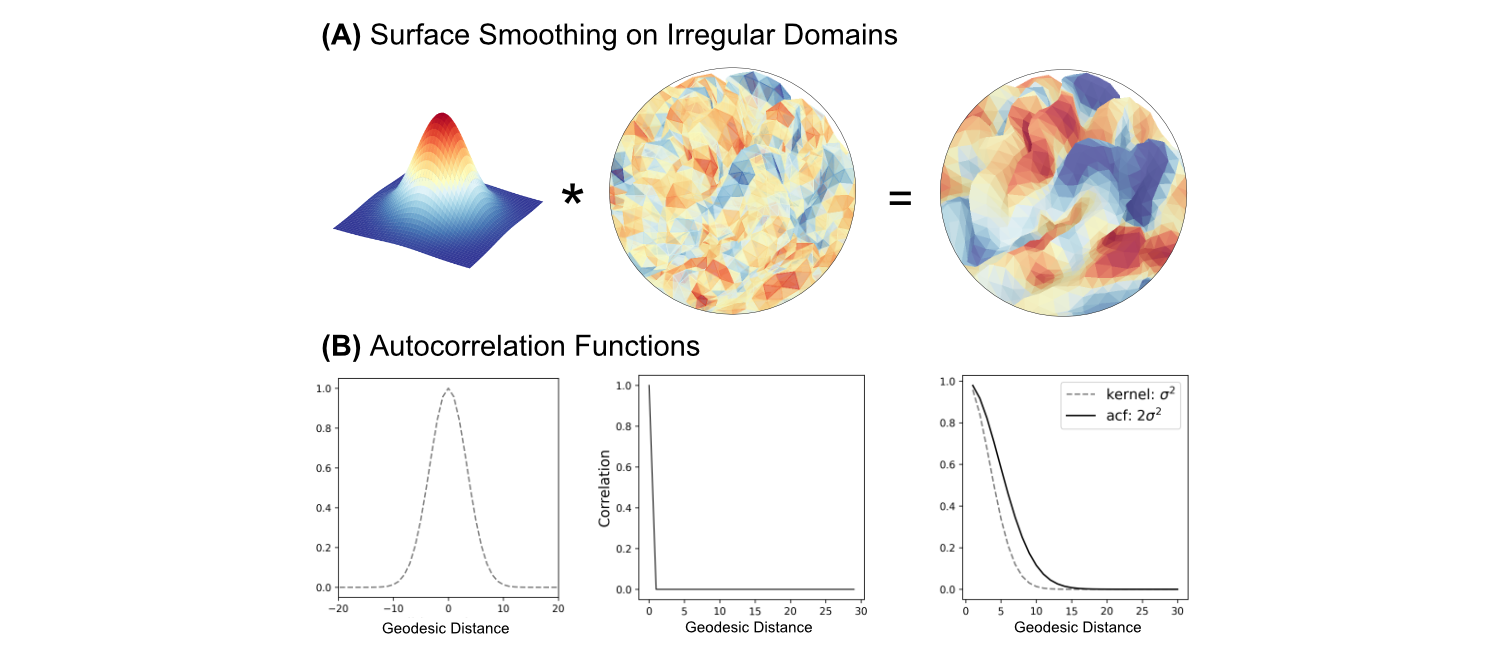
\includegraphics[width=0.9\linewidth]{project/figures/fig03.png}
    \caption{
    \textbf{(A)} Surface smoothing on irregular domains like cortical surfaces requires adapting the shape of the smoothing kernel to the intrinsic geometry of the manifold, as geodesic distances vary nonlinearly across folded regions. This figure demonstrates that convolution with a geodesic-based heat kernel transforms uncorrelated noise into a smooth random field.
    \textbf{(B)} First plot: the weights of the heat kernel decay exponentially with geodesic distance, reflecting how cortical smoothing prioritizes anatomically nearby regions. Second plot: the ACF of uncorrelated noise shows no correlation between points of nonzero distance, confirming spatial independence. Third plot: the ACF of the smoothed field matches exactly the shape of the kernel with double the bandwidth ($2\sigma$) demonstrating how convolution introduces spatially structured correlations.
    }
    \label{fig:surface-smoothing}
\end{figure}

\subsection{Method}

Following the description in \citet{seo_heat_2010}, the additive noise model:
\begin{align}\label{eq:Y(p)}
    Y(p) = \theta(p) + \epsilon(p), \quad \epsilon(p) \overset{\text{iid}}{\sim} \mathcal{N}(0, \mathbb{I})
\end{align}

\noindent defines data on a manifold $\mathcal{M} \subset \mathbb{R}^3$, where $Y$ represents the observed data, $\theta(p)$ is the signal, and $\epsilon(p)$ is Gaussian white noise. \\

The Laplace-Beltrami eigenvalue problem:
\begin{align}
    \Delta \psi_j = -\lambda \psi_j
\end{align}

\noindent defines the eigen decomposition of the Laplace-Beltrami operator $\Delta$ on $\mathcal{M}$. Solving this problem yields a sequence of eigenvalues $0 = \lambda_0 \leq \lambda_1 \leq \lambda_2 \leq \ldots$ and corresponding eigenfunctions $\psi_0, \psi_1, \psi_2, \ldots$ that form an orthonormal basis. Lower-order eigenfunctions capture global (low frequency) manifold features, while higher-order ones represent local (high-frequency) details.\\

The heat kernel:
\begin{align}\label{eq:heat-kernel}
     K_{\sigma}(p, q) = \sum_{j=0}^\infty e^{-\lambda_j\sigma} \psi_j(p) \psi_j(q)
\end{align}

\noindent defines the solution to the heat equation on the manifold, where the parameter $\sigma$ controls the smoothing bandwidth. The heat kernel is a probability distribution with respect to points $p, q$ and it respects the geometric structure of the underlying surface, which is a generalization of the Gaussian kernel for irregular domains.\\

Heat kernel smoothing:
\begin{align}
    Y_\sigma(p) \equiv K_{\sigma}  \ast Y(p) = \sum_{j=0}^\infty e^{-\lambda_j \sigma} \beta_j \psi_j(p)
\end{align}

\noindent is the convolution of the heat kernel with the data defined on the manifold. The coefficients  $\beta_j = \langle Y, \psi_j \rangle$ represent the projection of the signal from \eqref{eq:Y(p)} onto each eigenfunction. This analytical formulation provides an explicit series expansion that solves isotropic heat diffusion on the manifold.

\section{Paper Implementation}
\subsection{Method Simplification}
We can simplify heat kernel smoothing to the specific case of this project, where we are only smoothing white noise without any underlying signal,  $\theta(p) = 0$ from \eqref{eq:Y(p)}. The additive noise model simplifies to:

\begin{align}
Y(p) = \epsilon(p), \quad \epsilon(p) \overset{\text{iid}}{\sim} \mathcal{N}(0, \mathbb{I})
\end{align}

\noindent When projecting this white noise onto the Laplace-Beltrami eigenfunctions, we get:
\begin{align}
z_j \equiv \beta_j = \langle Y, \psi_j \rangle = \langle \epsilon, \psi_j \rangle \overset{iid}{\sim} \mathcal{N}(0, 1)
\end{align}

\noindent This simplification occurs because projecting spatially independent Gaussian noise onto an orthonormal basis yields independent standard normal random variables.\\

The heat kernel smoothed white noise is therefore:
\begin{align}
Y_\sigma(p) = \sum_{j=0}^\infty e^{-\lambda_j \sigma} z_j \psi_j(p)
\end{align}

\noindent which shows that heat kernel smoothing creates a random field where each spatial frequency component is dampened by the factor $e^{-\lambda_j \sigma}$. Higher frequencies (larger $\lambda_j$) are attenuated more strongly, producing a smooth field with controlled spatial correlation. The bandwidth parameter $\sigma$ determines the ACF of the resulting field, offering a principled method for generating random fields with specific autocorrelation properties on manifolds.

\subsection{Statistical Properties}
Given the simplification above, we can write the following statistical properties of the smoothed field, $Y_\sigma(p)$.\\

The mean of the smoothed field:
\begin{align}
    \mathbb{E}[Y_\sigma(p)] = 0
\end{align}

\noindent because heat diffusion conserves the underlying signal, which is zero in the case of white noise \citep{kushnarev_heat_2019}.\\

The variance of the smoothed field:
\begin{align}
    \mathbb{V}[Y_\sigma(p)] = \sum_{j=0}^\infty e^{-2\sigma\lambda_j}
\end{align}

\noindent is the sum of exponentially weighted terms determined by the Laplace-Beltrami eigenvalues. As $\sigma$ increases, high-frequency component (larger $\lambda_j$ values) are damped more strongly, reducing overall variability \citep{kushnarev_heat_2019}.\\

The covariance between points:
\begin{align}\label{eq:cov}
    \mathbb{C}[Y_\sigma(p), Y_\sigma(q)] = \sum_{j=0}^\infty e^{-\lambda_j 2\sigma} \psi_j(p) \psi_j(q).
\end{align}

\noindent This elegant result reveals that the covariance structure of the smoothed field is mathematically identical to the heat kernel \eqref{eq:heat-kernel} with bandwidth $2\sigma$ \citep{chung_discrete_2018}. This fundamental relationship demonstrates how the ACF of smoothed white noise precisely mirrors the kernel shape but with doubled bandwidth. Such correspondence allows for generating and analyzing smooth random fields on brain surfaces with precisely controlled spatial correlation structures. This property is particularly valuable for simulation studies validating statistical methods in neuroimaging, where understanding the spatial autocorrelation of noise is essential for proper inference.

\subsection{Underlying Graphs}
\begin{figure}[H]
    \centering
    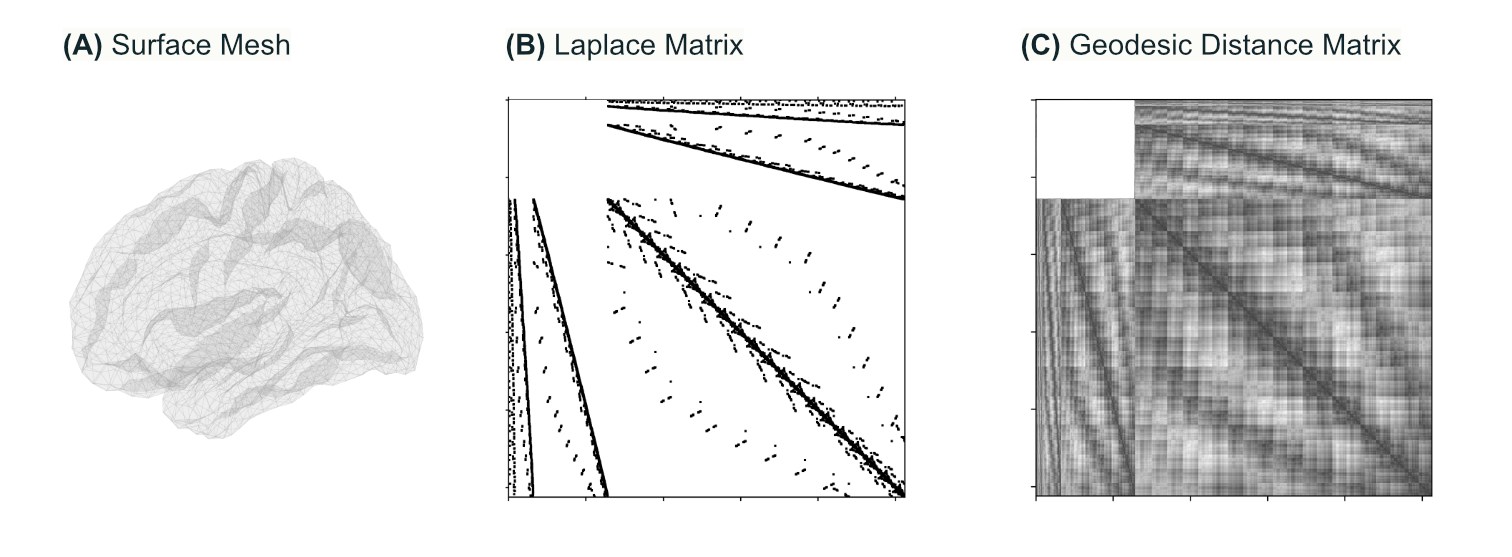
\includegraphics[width=0.9\linewidth]{project/figures/fig04.png}
    \caption{
    \textbf{(A)} Population-average FreeSurfer pial surface mesh ($\sim$40k vertices, $\sim$80k triangles, left hemisphere) representing cortical geometry. 
    \textbf{(B)} The Laplace matrix encoding surface connectivity: off-diagonals indicate adjacency between vertices, diagonals represent inverse vertex degrees (excluding the medial wall between hemispheres).
    \textbf{(C)} Geodesic distance matrix computed between all vertex pairs (excluding the medial wall between hemispheres).
    }
    \label{fig:surface-graphs}
\end{figure}

The Laplace-Beltrami operator is discretized on triangle meshes through the graph Laplacian matrix (Figure \ref{fig:surface-graphs}). For cortical surfaces with thousands of vertices, this sparse matrix encodes mesh connectivity: off-diagonal elements represent adjacent vertices with weights determined by local geometry, while diagonal elements contain the negative degrees of each vertex. This discretization preserves essential properties of the continuous operator while enabling numerical computation.\\

The eigenfunctions of this operator serve as what \citet{reuter_laplacebeltrami_2006} term "Shape-DNA" -- a signature of the manifold's intrinsic geometry. The LaPy Python package by the same authors enables efficient implementation of the graph Laplacian and its eigendecomposition, through sparse matrix storage and algorithms, allowing the computation of hundreds of eigenfunctions on high-resolution meshes. Further, we can also compute a matrix of geodesic distances between all vertex pairs, which is fundamental for estimating spatial ACFs. By binning pairs of vertices according to their geodesic separation distances, we can compute the correlation between data values as a function of distance along the surface. The geodesic distance matrix thus forms the critical link between the graph representation of the surface and the statistical properties of spatial processes defined on it.

\newpage
\subsection{Simulation Setting}
\begin{figure}[!ht]
    \centering
    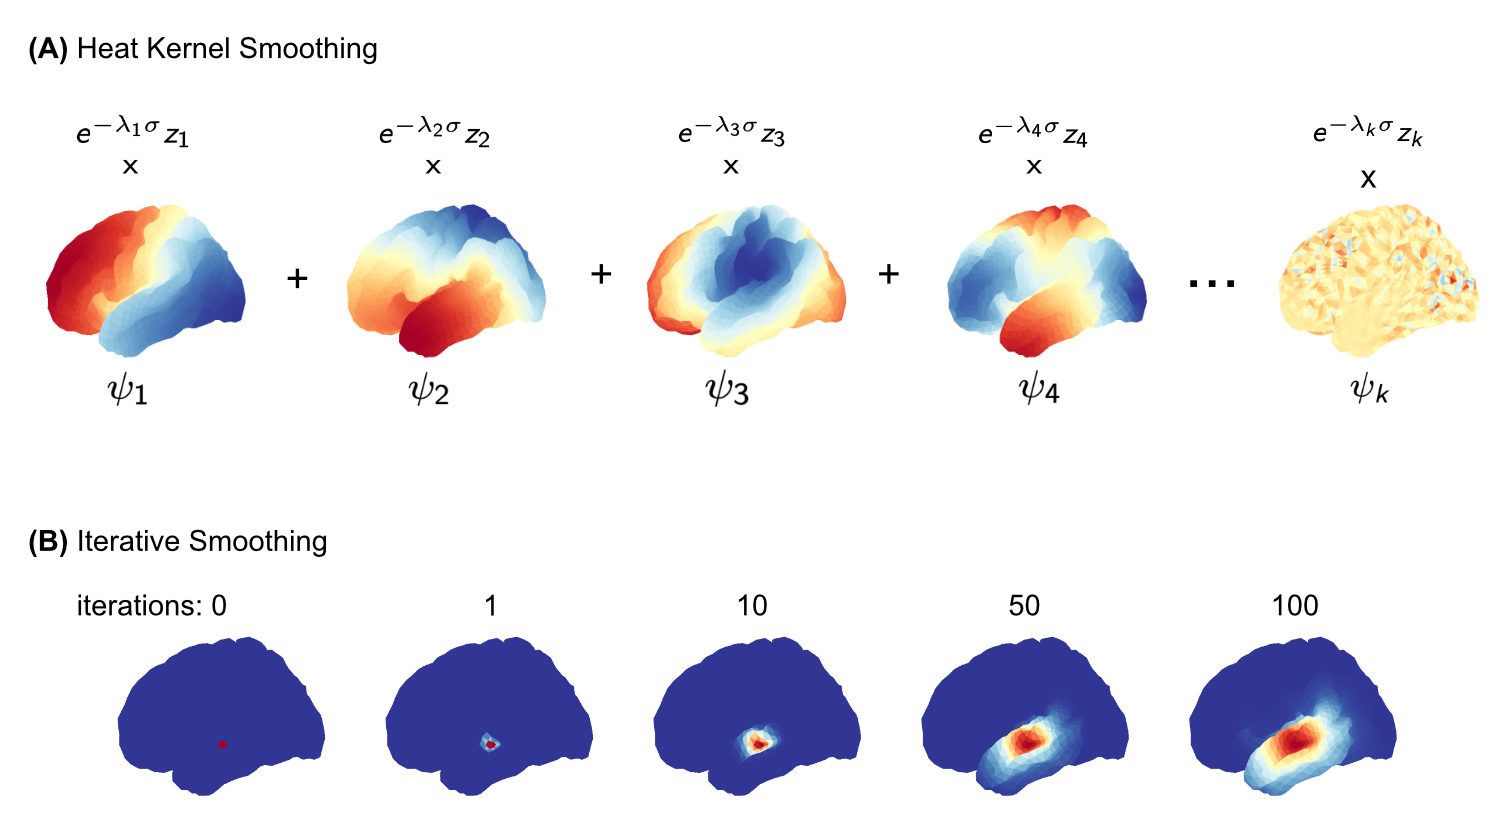
\includegraphics[width=0.9\linewidth]{project/figures/fig05.png}
    \caption{
    \textbf{(A)} Heat kernel smoothing on cortical surfaces. Laplace-Beltrami eigenfunctions $\psi_{1, 2, \dots, k}$ (truncated at $k=1000$) represent spatial frequencies of cortical geometry. Gaussian white noise $z_{1, 2, \dots, k}$ in the frequency domain is exponentially weighted by $e^{-\sigma\lambda_{1, 2, \dots, k}}$ (bandwidth $\sigma$), then linearly combined with $\psi_{1, 2, \dots, k}$ to construct smooth random fields with analytically known covariance structures.
    \textbf{(B)} Iterative nearest-neighbor smoothing on cortical surfaces. Uncorrelated noise is smoothed iteratively by averaging values at neighboring vertices on the cortical mesh, with the smoothing effect accumulating over multiple iterations. This example shows how a delta function (zeros except for a single vertex set to one) diffuses to neighboring vertices via repeated local averaging. 
    }
    \label{fig:simulation-setting}
\end{figure}

Figure \ref{fig:simulation-setting} contrasts two distinct approaches to spatial smoothing on the cortical surface. Panel A shows heat kernel smoothing via the Laplace-Beltrami eigenfunctions, or "Shape-DNA" of the underlying surface \citep{seo_heat_2010, reuter_laplacebeltrami_2006}. By truncating the eigenfunction expansion at $k=1000$, this method preserves the decomposition of spatial patterns from coarse to fine wavelengths, while being computationally tractable. Panel B illustrates the iterative nearest-neighbor smoothing. While methodologically straightforward, the theoretical basis for this method is unclear, especially in how local averaging converges to some type of random field, or if errors are introduces that propagate over iterations. 

\subsection{Simulation Results}
\begin{figure}[!ht]
    \centering
    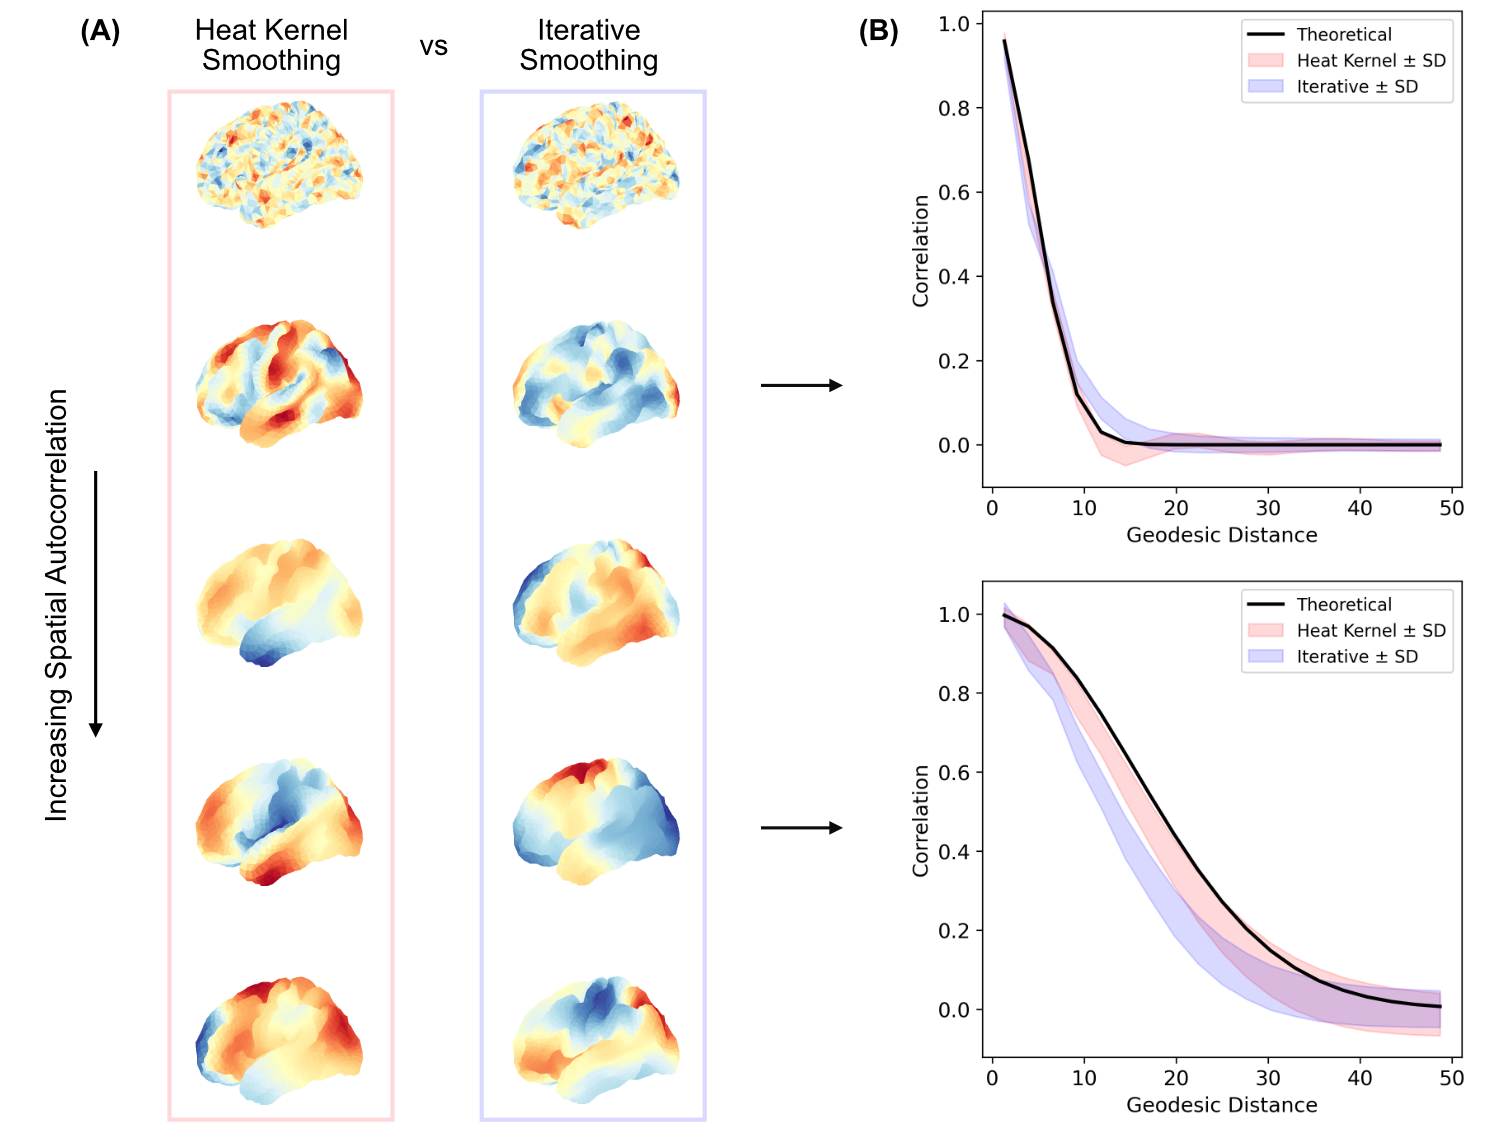
\includegraphics[width=0.9\linewidth]{project/figures/fig06.png}
    \caption{
    Comparison of heat kernel and iterative smoothing on cortical surfaces.
    \textbf{(A)} Smoothed random fields generated by heat kernel ($\sigma$: 0-500) and iterative methods (iterations: 1-100), showing increasing spatial autocorrelation. 
    \textbf{(B)} Theoretical (black) versus empirical ACFs ($n=$ 1000 simulations; heat kernel: blue $\pm$ SD; iterative: red $\pm$ SD). At low autocorrelation ($\sigma$=5, iterations=2) the heat kernel exhibits lower RMSE (0.018 vs 0.038). At high autocorrelation ($\sigma$=50, iterations=10), both methods are biased downward, while the heat kernel is relatively more accurate with RMSE (0.05 vs 0.09).
    }
    \label{fig:simulation-results}
\end{figure}

Figure \ref{fig:simulation-results} validates the theoretical advantages of heat kernel smoothing over iterative smoothing. It demonstrates that heat kernel smoothing produces spatially structured fields whose autocorrelations change with $\sigma$, consistent with the theoretical covariances from \eqref{eq:cov}. Likewise, although performing worst in terms of RMSE, the iterative kernel smoothing method is surprisingly close to the theoretical ACF. This might suggest that the repeated local averaging converges to some underlying random field, similar to that of heat kernel smoothing. Finally, the downward bias of both methods at maps with high autocorrelation points to unresolved issues in the implementation or theory. 

\newpage
\section{Conclusions}

Heat kernel smoothing as introduce by \citet{seo_heat_2010} offers significant advantages for processing data on complex anatomical surfaces by properly accounting for geodesic distances and intrinsic geometry. Our simulations demonstrate that the Laplace-Beltrami eigenfunction approach produces smooth random fields with autocorrelations that closely match theoretical results. The method's analytical formulation provides explicit control over spatial correlation structures through the bandwidth parameter $\sigma$.\\

While heat kernel smoothing outperforms iterative nearest-neighbor methods in terms of RMSE, the surprisingly close approximation achieved by iterative smoothing suggests potential convergence properties that warrant further investigation. Both methods exhibit downward bias at high autocorrelation levels, pointing to implementation challenges that remain unresolved. For heat kernel smoothing, this bias likely stems from eigenfunction truncation, while for iterative smoothing, it may reflect accumulated errors.\\

This work demonstrates the practical value of spectral methods for neuroimaging applications, particularly for simulation studies requiring precise control over spatial correlation structures. Future research should address the theoretical relationship between iterative and spectral approaches, evaluate truncation criteria for eigenfunction expansions, and optimize computational efficiency. Advancing these techniques will improve both the accuracy of surface-based analyses and the validity of statistical inference in neuroimaging research.

\section{Project Code}
\href{https://github.com/griegner/dsc190}{https://github.com/griegner/dsc190}

\bibliography{project/zotero}

\end{document}